%%%%%%%%%%%%%%%%%%%%%%%%%%%%%%%%

\documentclass[11pt,a4paper]{article}
\usepackage{times}
\usepackage[utf8]{inputenc}
\usepackage[croatian]{babel}
\usepackage[T1]{fontenc} % Latin Modern

%%%%%%%%%%%%%%%%%%%%%%%%%%%%%%%%


%%%%%%%%%%%%%%%%%%%%%%%%%%%%%%%%
%%%%%%%%  MATEMATICKI PAKETI %%%%%%%%%%%
%%%%%%%%%%%%%%%%%%%%%%%%%%%%%%%%

\usepackage{amsmath}
\usepackage{amsfonts}
\usepackage{amssymb}
\usepackage{esvect}
\usepackage{bm}

%%%%%%%%%%%%%%%%%%%%%%%%%%%%%%%%

%%%%%%%%%%%%%%%%%%%%%%%%%%%%%%%%
%%%%%%%%%% PAKETI ZA SLIKE  %%%%%%%%%%%%
%%%%%%%%%%%%%%%%%%%%%%%%%%%%%%%%

\usepackage{graphicx}
\usepackage{float}
\usepackage[hidelinks]{hyperref}
\usepackage{caption}
\usepackage{subcaption}
\usepackage{booktabs}

%%%%%%%%%%%%%%%%%%%%%%%%%%%%%%%%

%%%%%%%%%%%%%%%%%%%%%%%%%%%%%%%%
%%%%%%%%%    PRORED 1.5   %%%%%%%%%%%%%%
%%%%%%%%%%%%%%%%%%%%%%%%%%%%%%%%

\renewcommand{\baselinestretch}{1.5}

%%%%%%%%%%%%%%%%%%%%%%%%%%%%%%%%


%%%%%%%%%%%%%%%%%%%%%%%%%%%%%%%%
%%%%%%%%%% TABLICA - ANTUN %%%%%%%%%%%%
%%%%%%%%%%%%%%%%%%%%%%%%%%%%%%%%

\usepackage{array}
\usepackage{multirow}
\newcolumntype{C}[1]{>{\centering\let\newline\\\arraybackslash\hspace{0pt}}m{#1}}
\newcolumntype{L}[1]{>{\raggedright\let\newline\\\arraybackslash\hspace{0pt}}m{#1}}
\newcolumntype{R}[1]{>{\raggedleft\let\newline\\\arraybackslash\hspace{0pt}}m{#1}}
\usepackage{ctable}

%%%%%%%%%%%%%%%%%%%%%%%%%%%%%%%%

%%%%%%%%%%%%%%%%%%%%%%%%%%%%%%%%
%%%%%%%%%% TABLICA - MARTINA %%%%%%%%%%%
%%%%%%%%%%%%%%%%%%%%%%%%%%%%%%%%

\makeatletter
\renewcommand*\env@matrix[1][\arraystretch]{%
  \edef\arraystretch{#1}%
  \hskip -\arraycolsep
  \let\@ifnextchar\new@ifnextchar
  \array{*\c@MaxMatrixCols c}}
\makeatother



%%%% LATEX KOD ZA KORISTENJE TABLICE %%%%
%%% PRIMJER %%%

%\setlength\extrarowheight{1pt}
%\begin{table}[h]
%\centering
%\caption{Tablica s prikazom }
%\label{prva}
%\begin{tabular}{|l|c|}
%\hline
%\textbf{txt} &  \\ \hline 
%txt & txt    \\ 
%txt & txt   \\ \hline
%txt & txt    \\ \hline
%\end{tabular}
%\end{table}

%%%%%%%%%%%%%%%%%%%%%%%%%%%%%%%%


%%%%%%%%%%%%%%%%%%%%%%%%%%%%%%%%
%%%%%%% DIO ZA UNOS ISJECAKA KODA %%%%%%%%
%%%%%%%%%%%%%%%%%%%%%%%%%%%%%%%%

\usepackage{listings}
\usepackage{color}
 
\definecolor{codegreen}{rgb}{0,0.6,0}
\definecolor{codegray}{rgb}{0.5,0.5,0.5}
\definecolor{codepurple}{rgb}{0.58,0,0.82}
 
\lstdefinestyle{mystyle}{   
    commentstyle=\color{codegreen},
    keywordstyle=\color{blue},
    numberstyle=\tiny\color{codegray},
    stringstyle=\color{codepurple},
    basicstyle=\footnotesize,
    breakatwhitespace=false,         
    breaklines=true,                 
    captionpos=b,                    
    keepspaces=true,                 
    numbers=left,                    
    numbersep=5pt,                  
    showspaces=false,                
    showstringspaces=false,
    showtabs=false,                  
    tabsize=1
}
 
\lstset{style=mystyle}

%\lstinputlisting[language=Matlab, firstline=1, lastline=4, numbers=left, frame=single, label={lst:prvi}, caption={Diskretizacija sustava korištenjem Matlaba}, captionpos=b]{peti.m} 

%%%%%%%%%%%%%%%%%%%%%%%%%%%%%%%%


%----------------------------
% za uredjenje stranice
\usepackage[left=2.5cm,right=2.5cm,top=2.5cm,bottom=2.5cm]{geometry}
\usepackage{fancyhdr}
\pagestyle{fancy} 
\lhead{\leftmark}
\rhead{\rightmark}
\usepackage{titlesec} %za točku iza broja sectiona
\titleformat{\section}{\huge\bfseries}{\thetitle.\quad}{0em}{}
\titleformat{\subsection}{\LARGE\bfseries}{\thetitle.\quad}{0em}{}
\titleformat{\subsubsection}{\Large\bfseries}{\thetitle.\quad}{0em}{}
\titleformat{\paragraph}
{\normalfont\large\bfseries}{\thetitle.\quad}{1em}{}
\titlespacing*{\paragraph}
{0pt}{3.25ex plus 1ex minus .2ex}{1.5ex plus .2ex}
\setcounter{secnumdepth}{5}

\usepackage{indentfirst} %uvlacenje prvog paragrafa
% primjer pozivanja sectiona
% \section*{UVOD} \pdfbookmark{UVOD}{section:UVOD}

\usepackage{tocloft}
\usepackage{import}
\usepackage{standalone}
\graphicspath{{figures/}} 

\hypersetup{
  colorlinks   = true, %Colours links instead of ugly boxes
  urlcolor     = black, %Colour for external hyperlinks
  linkcolor    = black, %Colour of internal links
  citecolor   = blue %Colour of citations
}

\usepackage{subcaption}
\usepackage{lscape}
\begin{document}

U sklopu ovog poglavlja dan je pregled nelinearnog matematičkog modela letjelice koji opisuje njezinu rotaciju i translaciju. Na temelju tog modela obavlja se njegova linearizacija u svrhu dobivanja prijenosne funkcije sustava koja se potom koristi za upravljanje. Potpuni model nalazi se u literaturi \cite{haus3}.

\medskip

\subsection{Nelinearni dinamički model letjelice s pokretnim masama}

Koordinatni sustav letjelice prikazan je Slikom \ref{fig:mod}. Svi vektori korišteni za opis ovog sustava, uz iznimku sile gravitacije, izraženi su u lokalnom mobilnom koordinatnom sustavu letjelice označenom s $L_{0}$. Vektor sile gravitacije prikladno je izražen u globalnom nepomičnom koordinatnom sustavu $L_{I}$. $L_{CoG}$ označava koordinatni sustav vezan za centar mase letjelice te je on usklađen s $L_{0}$ koordinatnim sustavom.


\begin{figure}[H]
	\centering
	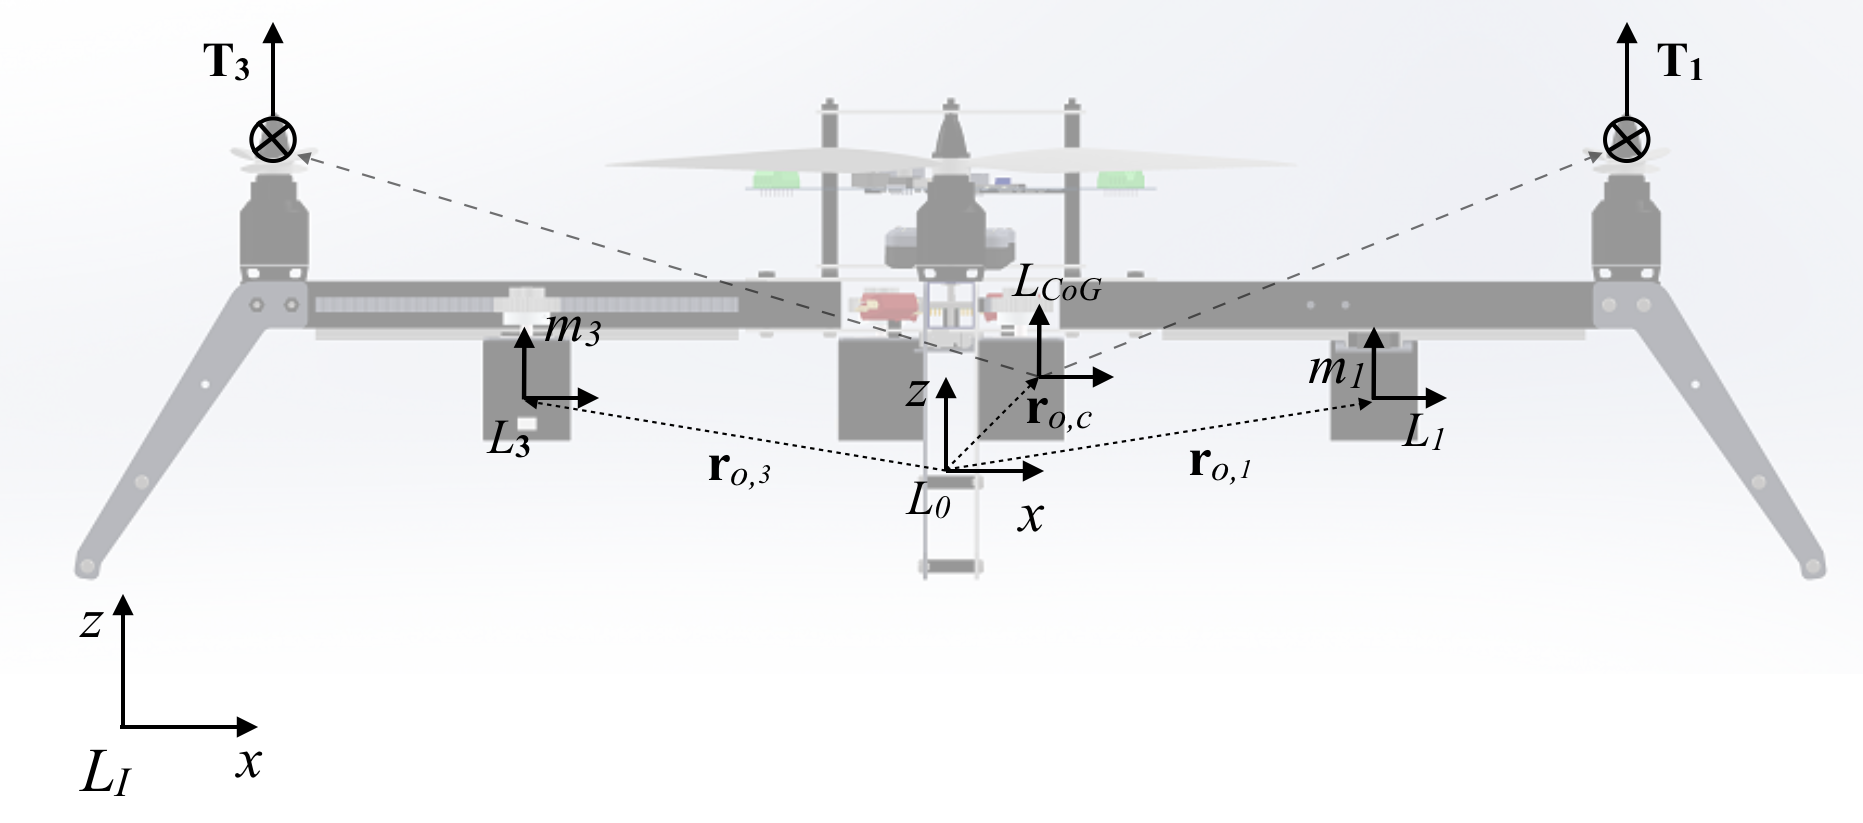
\includegraphics[scale=0.23]{model}
	\caption{Koordinatni sustav letjelice}
	\label{fig:mod}
\end{figure}

Matematičko modeliranje započinje se standardnim zapisom formule za proizvoljni vektor promjenjive duljine izražen u lokalnom mobilnom koordinatnom susavu letjelice ($L_{0}$):

\begin{equation}
\frac{d^{\omega}}{dt}({r}_{0}) =  {\dot{r}}_{0} + {\omega} \times {r}_{0} 
\label{eq:r0}
\end{equation}

gdje $\boldsymbol{\dot{r}_{0}}$ označa vektor stope promjene u $L_{0}$ koordinatnom sustavu, dok $\omega$  označava kutnu brzinu gibanja letjelice, odnosno kutnu brzinu gibanja $L_{0}$ koordinatnog sustava. Bitno je napomenuti kako $\frac{d^{\omega}}{dt}$ označava vremensku derivaciju vektora izraženog u mobilnom koordinatnom sustavu letjelice s obzirom na globalni koordinatni sustav. 

\medskip

Centar mase letjelice promatran iz lokalnog koordinatnog sustava dan je sljedećim izrazom:

\begin{equation}
 {r}_{0,c} = \frac{ {m}_{b} {r}_{0,b} + \sum_{i=1}^{4}{m}_{i} {r}_{0,i}}{{m}_{b} + \sum_{i=1}^{4} {m}_{i}} = \frac{\sum_{i=1}^{4} {m}_{i} {r}_{0,i}}{ {M}}
\label{eq:r0c}
\end{equation}

\medskip

gdje je s $m_{b}$ označena masa krutog tijela letjelice bez masa. Masa pomične mase označena je s $m_{i}$, dok je s $M$ označena ukupna masa cijele letjelice. $r_{0,i}$ označava poziciju $i$-te mase, dok $r_{0,b}$ označava poziciju tijela letjelice te je jednak 0. $r_{0,b} = 0$ zbog početne pretpostavke koja nalaže kako se ishodište mobilnog koordinatnog sustava letjelice podudara s koordinatnim sustavom centra mase krutog tijela letjelice. 

\medskip

Koristeći prethodni izraz izražava se brzina koordinatnog sustava centra mase $v_{c}$ s obzirom na globalni koordinatni sustav:
\begin{equation}
 {v_{c} = v_{0} + v_{0,c} + \omega \times r_{0,c}}
\label{eq:vc}
\end{equation}

gdje su redom $v_{0}$ brzina $L_{0}$ koordinatnog sustava s obzirom na $L_{I}$ i $v_{0,c}$ brzina $L_{CoG}$ koordinatnog sustava s obzirom na $L_{0}$. Analogno (\ref{eq:vc}) slijedi izraz za brzinu $i$-te pomične mase $v_{i}$:
\begin{equation}
 {v_{i} = v_{0} + v_{0,i} + \omega \times r_{0,i}}
\label{eq:vi}
\end{equation}

Prethodni izraz (\ref{eq:vi}) moguće je proširiti uvrštavanjem izraza (\ref{eq:vc}), te na taj način izraziti brzinu pokretne mase $i$ kao funkciju brzine $v_{c}$: 
\begin{equation}
 {v_{i} = v_{c} + v_{0,i} - v_{0,c} + \omega \times r_{c,i}}
\label{eq:vi2}
\end{equation}

$v_{0,i}$ označava relativnu brzinu $i$-te mase, $r_{c,i}$ označava poziciju $i$-te mase u $L_{CoG}$ koordinatnom sustavu, dok se $v_{0,c}$ računa prema (\ref{eq:v0c}):
\begin{equation}
 {v_{0,c} = \frac{\sum_{i=1}^{4}m_{i}\dot{r}_{0,i}}{M}}
\label{eq:v0c}
\end{equation}

Prema definiciji \cite{ilijic}, vremenska derivacija linearnog momenta (\ref{eq:Li}) jednaka je zbroju svih vanjskih sila koje djeluju na česticu sustava, odnosno na $i$-tu pokretnu masu (\ref{eq:Lidot}). 
\begin{equation}
 {L_{i} = m_{i} \cdot v_{i}}
\label{eq:Li}
\end{equation}

\begin{equation}
 {\frac{d^{\omega}}{dt} L_{i} = \sum_{k=1}^{3}f_{ik}}
\label{eq:Lidot}
\end{equation}

U slučaju ove bespilotne letjelice tri vanjske sile djeluju na pokretne mase:

\begin{enumerate}
 \item Sila motora koji upravlja pomakom masa:
\begin{equation}
f_{i1}  =K_{m}T_{r}U_{i}\left(\sin\left(\frac{\pi}{2}i\right) \bm{\hat{i}} - \cos\left( \frac{\pi}{2}i\right) \bm{\hat{j}}\right), i \in \{1,2,3,4\}
\label{eq:fi1}
\end{equation}

gdje je $K_{m}$ konstanta motora, $T_{r}$ prijenosni omjer a $U_{i}$ napon na motorima.  $\bm{\hat{i}}$ i  $\bm{\hat{j}}$ jedinični vektori u $L_{0}$ koordinatnom sustavu koji pokazuju redom u $x$ i $y$ smjeru.

\item Sila gravitacije:
\begin{equation}
f_{i2} = -m_{i}\cdot g \bm{\hat{K}}
\label{eq:fi2}
\end{equation}
gdje je  $\bm{\hat{K}}$ jedinični vektor u $L_{I}$ koordinatnom sustavu koji pokazuje u $z$ smjeru, dok je $g$ gravitacijska konstanta. 

\item Sila trenja modelirana je tako da bude proporcionalna brzini pokretne mase
\begin{equation}
f_{i3} = -c_{d} \cdot v_{0,i}
\label{eq:fi3}
\end{equation}

gdje je $c_{d}$ koeficijent trenja.

\end{enumerate}

Kombiniranjem izraza (\ref{eq:vi}) i (\ref{eq:Lidot}) slijedi izraz za linearnu akceleraciju $t$-te pomične mase:

\begin{equation}
\frac{d^{\omega}}{dt}v_{0,i} = \frac{1}{m_{i}}\left(\sum_{k=1}^{3}f_{ik}\right) - \frac{d^{\omega}}{dt} \left( v_{0} + \omega \times r_{0,i} \right) 
\label{eq:voidot}
\end{equation}

Slijedi modeliranje linearnog momenta cjelokupnog sustava. Prema definiciji vrijedi da je ukupan linearni moment sustava jednak zbroju linearnog momenta krutog tijela letjelice $L_{b}$ te linearnog momenta svake od pomičnih masa $L_{i}$:
\begin{equation}
L_{s} = L_{b} + \sum_{i=1}^{4}L_{i}
\label{eq:Ls}
\end{equation}

Koristeći izraze (\ref{eq:r0c}) i (\ref{eq:vi}), kao i činjenicu da je $v_{0,b} = 0$ slijedi:
\begin{equation}
L_{s} = M \cdot (v_{0} + \omega \times r_{0,c}) + \sum_{i=1}^{4}m_{i}c_{0,i} = M \cdot (v_{0} + \omega \times r_{0,c}) + \sum_{i=1}^{4}L_{0,i}
\label{eq:Ls2}
\end{equation}

Konačno, koristeći definiciju stope promjene linearnog momenta, slijedi izraz za ubrzanje krutog tijela letjelice:
\begin{equation}
\frac{d^{\omega}}{dt} v_{0} = \frac{1}{M} \left( \sum_{j=1}^{4} F_{rj} + F_{g} - \frac{d^{\omega}}{dt} \sum_{i=1}^{4}L_{0,i}  \right) - \frac{d^{\omega}}{dt} (\omega \times r_{0,c})
\label{eq:v0dot}
\end{equation}

Potisak motora te sila gravitacije su vanjske sile koje djeluju na cijeli sustav.

Sila potiska koju uzrokuje svaki rotor prikazana je kvaratnim izazom (\ref{eq:Frj}), gdje su $\Omega_{j}$ brzina $j$-tog rotora, $b_{f}$ konstanta motora, a  $\bm{\hat{k}}$ jedinični vektor u smjeru $z$ osi:
\begin{equation}
F_{rj} = b_{f}\Omega_{j}^{2} \bm{\hat{k}}
\label{eq:Frj}
\end{equation}


Uz pretpostavku upravljane brzine rotora, njezina zatvorena petlja opisana je sljedećim izrazom, gdje su $T_{r}$ vremenska konstanta rotora pogonjenog benzinskim motorom, a $\Omega_{r,j}$ referentna brzina rotora:
\begin{equation}
T_{r}\dot{\Omega}_{j} + \Omega_{j} = \Omega_{r,j}
\label{eq:omega_rj}
\end{equation}

Sila gravitacije izražena u globalnom koordinatnom sustavu $L_{I}$ jednaka je:
\begin{equation}
F_{g} = -Mg \bm{\hat{K}}
\label{eq:Fg}
\end{equation}


Sljedeći korak je modeliranje kutnog gibanja letjelice. Kreće se od definicije kutnog momenta izraženog u koordinatnom sustavu centra mase zajedno u kombinaciji s (\ref{eq:vi2}). Kutni moment cijelog sustava $H_{s}$ prikazan je sljedećim izrazom (\ref{eq:Hs}):
\begin{equation}
H_{s} = H_{b} + \sum_{i=1}^{4}H_{i}
\label{eq:Hs}
\end{equation}

$H_{b}$ označava kutni moment krutog tijela letjelice (bez pomičnih masa), te je jednak (\ref{eq:Hb}):
\begin{equation}
H_{b} = \int_{k} r_{c,k} \times (v_{k}dm_{k}) = \int_{k} r_{c,k} \times (v_{c} + v_{0,k} - v_{0,c} + \omega \times r_{c,k})dm_{k}
\label{eq:Hb}
\end{equation}

I konačno, $H_{i}$ označava kutni moment $i$-te mase:
\begin{equation}
H_{i} = \int_{ji} r_{c,ji} \times (v_{ji}dm_{ji}) = \int_{ji} r_{c,ji} \times (v_{c} + v_{0,i} - v_{0,c} + \omega \times r_{c,ji})dm_{ji}
\label{eq:Hi}
\end{equation}

$dm_{k}$ označava $k$-ti Infinitezimalni dio krutog tijela letjelice, dok $v_{k}$ označava njegovu brzinu, a $r_{c,k}$ vektor udaljenosti između centra mase tijela te $k$-tog dijela tijela. Prema definiciji je $v_{0,k} = 0$. 

Iz definicije momenta inercije u kombinaciji s (\ref{eq:r0c}) slijedi:
\begin{equation}
H_{s} = I_{s}^{c}\omega + \sum_{i=1}^{4}r_{c,i} \times L_{0,i}
\label{eq:Hs2}
\end{equation}

gdje je $I_{s}^{c}$ cjelokupni moment inercije sustava s obzirom na centar mase letjelice, te se može izražunati kao zbroj inercijskih doprinosa svakog dijela letjelice:
\begin{equation}
I_{s}^{c} = I_{b}^{c} + \sum_{i=1}^{4}I_{i}^{c}
\label{eq:Ics}
\end{equation}

$I_{b}^{c}$ označava moment inercije krutog tijela letjelice, dok $I_{i}^{c}$ označava moment inercije $i$-te pomične mase. Koristeći \textit{Steinerov teorem}, odnosno \textit{Teorem o paralelnim osima}, slijedi izraz za proračun momenata inercije pomičnih masa:
\begin{equation}
I_{i}^{c} = I_{i} + m_{i} \left(  r_{ci,}^{T} \cdot r_{c,i}E_{3} - r_{c,i}\cdot r_{c,i}^{T} \right)
\label{eq:Iic}
\end{equation}

gdje je s $I_{i}$ označen moment inercije $i$-tog dijela. Sljedeći izraz korišten je za izvođenje izraza za stopu promjene kutne brzine:
\begin{equation}
\frac{d^{\omega}}{dt} \left( I_{s}^{c} \omega + \sum_{i=1}^{4} r_{c,i}\times L_{0,i}  \right) = \sum_{j=1}^{4}(M_{fi} + M_{dj}) + M_{g}
\label{eq:dtM}
\end{equation}


Vanjski momenti koji djeluju na sustav letjelice te koji se sljedeći modeliraju su:
\begin{enumerate}
\item Moment koji stvaraju sile rotora na kraku
\begin{equation}
M_{fj} = r_{c,rj} \times F_{rj} = (r_{c,0} + r_{0,rj}) \times F_{rj}
\label{eq:Mfj}
\end{equation}

gdje je s $r_{0,rj}$ označen vektor koji se proteže od ishodišta letjelice do $j$-tog rotora.

\item Momenti rotora uzrokovani induciranim trenjem:

\begin{equation}
M_{dj} = \zeta_{j}b_{m}b_{f}\Omega_{j}^{2} \bm{\hat{k}}
\label{eq:Mdj}
\end{equation}

gdje je $b_{m}$ momentna konstanta propulzijskog sustava, $\zeta_{j} =  1$ ukoliko se $j$-ti propeler okreće u smjeru kazaljke na satu (propeleri 1 i 3), a $\zeta_{j} =  -1$ ukoliko se $j$-ti propeler okreće u smjerusuprotnom smjeru kazaljke na satu (propeleri 2 i 4).

\item Moment uzrokovan silom gravitacije
\begin{equation}
M_{g} = r_{c,b} \times (-m_{b}g \bm{\hat{K}}) + \sum_{i=1}^{4} \times (-m_{i}g \bm{\hat{K}})
\label{eq:Mg}
\end{equation}
\end{enumerate}

gdje su $r_{c,b}$ i $r_{c,i}$ pozicije letjelice i $i$-te pomične mase.

Pri opisu pozicije letjelice koriste se standardni Eulerovi kutevi. Za prelazak iz globalnog u lokalni koordinatni sustav letjelice koristi se pretpostavka da se letjelice prvo rotira oko $z$ osi za \textit{kut zakretanja} $\psi$, zatim da se rotira oko oko $y$ osi za \textit{kut naginjanja} $\theta$, te konačko da se rotira oko $x$ osi za \textit{kut kotrljanja} $\varphi$.



\subsection{Linearizirani dinamički model letjelice}

Svi sustavi koje susrećemo u praksi su nelinearni. Analiza i sinteza takvih sustava je vrlo složena, jer za razliku od linearnih sustava danas još ne postoji zaokružena teorija rješavanja nelinearnih diferencijalnih jednadžbi, koja bi davala opće rezultate za sve nelinearne sustave. Zbog toga su rješenja koja dobijemo za određeni nelinearni sustav svojstvena obično samo tom sustavu i ne mogu se proširiti na ostale nelinearne sustave. Međutim, nelinearni matematički model moguće je linearizirati ovisno o zadanom režimu rada. Linearizacijom nelinearnog sustava oko jednog ravnotežnog stanja dobiti će se linearni matematički model kojim će se dinamika nelinearnog sustava moći objasniti u okolini odabranog ravnotežnog stanja \cite{vukic}.

\medskip

Prethodno modelirani nelinearni dinamički model letjelice potrebno je stoga linearizirati u svrhu dobivanja prijenosne funkcije modela, koja opisuje stopu promjene kutne brzine gibanja letjelice s obzirom na promjenu pozicije pokretne mase. U nastavku je opisana analiza dinamike za \textit{kut poniranja}, ali s obzirom na simetričnost letjelice analogna analiza vrijedi i za \textit{kut valjanja}. 

\medskip

S obzirom da je linearizacija nelinearnih modela osjetljiv zadatak, potrebno je pomno odabrati početne uvjete, odnosno radnu točku oko koje će se obaviti linearizacija. Kao radna toča, odnosno početno stanje sustava letjelice, odabire se stanje u kojem letjelica lebdi na mjestu (\textit{hover condition}). To stanje podrazumijeva malu kutnu brzinu letjelice. Odabir ovog početnog stanja za posljedicu ima zanemarenje žiroskopskog i centrifugalnog efekta koji se javljaju pri analizi pokretnog referentnog okvira. 

\medskip

Nadalje, podrazumijeva se kako klizni mehanizam pokretnih masa osigurava $PT_{2}S$ odziv dinamike pozicije mase na zadanu pobudu. Istu je dinamiku potrebno identificirati za potrebe projektiranja upravljanja, što je obrađeno u sljedećem poglavlju ovog rada. Opći izraz $PT_{2}S$ člana jednak je izrazu (\ref{eq:pt2s}) u nastavku, gdje $\omega_{mm}$ i $\zeta_{mm}$ predstavljaju nazivnu frekvenciju i prigušenje sustava, a $x_{i}$ poziciju $i$-te mase u lokalnom koordinatnom sustavu:
\begin{equation}
\frac{x_{i}}{x_{i, ref}}(s) = \frac{1}{\frac{1}{\omega_{mm}^{2}}s^{2} + \frac{2\zeta_{mm}}{\omega_{mm}}s + 1 }
\label{eq:pt2s}
\end{equation}

Dinamikom $kuta \ poniranja \ \theta$ upravlja se isključivo pozicijama masa 1 i 3, jer one utječu na pomak centra mase letjelice u $x$ smjeru lokalnog koordinatnog sustava. U drugu ruku, dinamikom $kuta \ valjanja \ \varphi$ upravlja se masama 2 i 4, jer one utječu na pomak centra mase u $y$ smjeru lokalnog koordinatnog sustava. Njihove pozicije dane su izrazima (\ref{eq:r0i}) i (\ref{eq:r0j}), gdje $\frac{L}{2}$ označava početnu poziciju pokretne mase, $x_{1}$ i $x_{3}$ pomake masa 1 i 3 u $x$ smjeru, a $y_{2}$ i $y_{4}$ pomake masa 2 i 4 u $y$ smjeru. $z_{m}$ označava konstantni pomak svih masa u $z$ smjeru.
\begin{equation}
r_{0,i} = \left[
\begin{matrix}
\sin\left(\frac{\pi}{2}i\right)\frac{L}{2} + x_{i} & 0 & z_{m}
\end{matrix} \right] ^{T}, i \in \{ 1, 3\}
\label{eq:r0i}
\end{equation}

\begin{equation}
r_{0,j} = \left[
\begin{matrix}
0 & -\cos\left(\frac{\pi}{2}j\right)\frac{L}{2} + y_{j} & z_{m}
\end{matrix} \right] ^{T}, j \in \{ 2, 4\}
\label{eq:r0j}
\end{equation}

 
Sljedeći izraz opisuje centar mase s obzirom na lokalni koordinatni sustav letjelice te nastaje uvrštavanjem izraza (\ref{eq:r0i}) i (\ref{eq:r0j}) u (\ref{eq:r0c}):
\begin{equation}
r_{0,c} = \mu \cdot \left[
\begin{matrix}
(x_{1} + x_{3}) & (y_{2} + y_{4}) & 4z_{m}
\end{matrix} \right]^{T}
\label{eq:r0c}
\end{equation}

gdje je $\mu = \frac{m}{M}$. Pozicija rotora u lokalnom koordinatnom sustavu opisana je s:
\begin{equation}
r_{0,rj} = \left[
\begin{matrix}
sin\left(\frac{\pi}{2}j\right)L & -\cos\left(\frac{\pi}{2}j\right)L & z_{r}
\end{matrix} \right] ^{T}, j \in \{ 1, 2, 3, 4\}
\label{eq:r0rj}
\end{equation}

gdje $z_{r}$ označava vertikalni odmak rotora od ishodišta koordinatnog sustava $L_{0}$. Koristeći izraze (\ref{eq:Mfj}),(\ref{eq:r0c}) i (\ref{eq:r0rj}) slijedi izraz koji opisuje momente proizvedene od strane sila rotora:
\begin{equation}
\sum_{j=1}^{4}M_{fj} = \left[
\begin{matrix}
(F_{r,2} - F_{r,4})L & (F_{r,3} - F_{r,1})L & L
\end{matrix}\right]^{T} + \sum_{j=1}^{4}F_{r,j} 
\left[\begin{matrix}
-\mu(y_{2} + y_{4}) & \mu(x_{1} + x_{3}) & 0
\end{matrix}\right]^{T}
\label{eq:sumaMfj}
\end{equation}

gdje $F_{r,j}$ označava magnitudu sile $j$-tog rotora. 

\medskip

Proširenjem izraza (\ref{eq:dtM}) može se izlučiti izraz za kutnu brzinu u smjeru $y$ osi dobije se sljedeći izraz:
\begin{equation}
\begin{split}
I_{yy}\dot{\omega}_{y}  & = \sum_{j=1}^{4}M_{fj}\cdot  \bm{\hat{j}} - (I_{xx} - I_{zz})\omega_{x}\omega_{z} \\
&- 2m_{b}\mu^{2}(x_{1} + x_{3})(\dot{x}_{1} + \dot{x}_{3} )\omega_{y} \\
&- 2m\frac{l}{2}(\dot{x}_{1} - \dot{x}_{3})\omega_{y} \\
&- 2m(\dot{x}_{1}x_{1} + \dot{x}_{3}x_{3})(1-2\mu + 2\mu^{2})\omega_{y} \\
&+ 4m(\dot{x}_{1}x_{3} + \dot{x}_{3}x_{1})\mu(1-\mu)\omega_{y} \\
&+ m \omega_{z}(\dot{y}_{2} + \dot{y}_{4})z_{m}(1-4\mu) \\
&+ m\omega_{x}\mu ((y_{2} + y_{4})(\dot{x}_{1} + \dot{x}_{3})-(\dot{y}_{2} + \dot{y}_{4})(x_{1} + x_{3})) \\
&- m(\ddot{x}_{1} + \ddot{x}_{3})z_{m}(1 - 4\mu)
\end{split}
\label{eq:Iyyw}
\end{equation}

gdje su $I_{xx}$, $I_{yy}$ i $I_{zz}$ nominalni momenti inercije u $x$, $y$ i $z$ smjeru, te su proračunati za početne pozicije pomičnih masa, smještenih u centru kraka letjelice. Drugi dio izraza u (\ref{eq:Iyyw}) rezultat je žiroskopskog efekta, treći, četvrti, peti i šesti dio izraza proizlaze iz promjene momenta inercije, dok su sedmi i osmi dio izraza rezultat $\omega \times \sum_{i=1}^{4} = r_{c,i}\times L_{0,i}$ projeciranog na $y$ os, a deveti dio izraza jednak je $y$ komponenti od $\sum_{i=1}^{4}r_{c,i}\times \dot{L}_{0,i}$.  

\medskip

Krajnji cilj dobivanja prijenosne funkcije sustava svodi se na dizajniranje upravljanja za jedan takav sustav, stoga se u model uvodi upravljački signal $u$. S obzirom da prikazujemo dinamiku \textit{kuta poniranja}, taj je upravljački signal jednak referentnim vrijednostima za poziciju masa 1 i 3:

\begin{equation}
 u_{\theta} = x_{1, ref} = x_{3, ref}
 \label{eq:u}
 \end{equation} 

Konačno, prijenosna funkcija slijedi iz (\ref{eq:pt2s}), (\ref{eq:u}), (\ref{eq:sumaMfj}) te drugog i devetog dijela izraza (\ref{eq:Iyyw}) (jer iz njih proizlazi dominantan dinamika kuta valjanja u početnom stanju lebdjenja) \cite{haus2} \cite{haus3}:

\begin{equation}
\boxed{
\frac{\omega_{y}(s)}{u_{\theta}(s)} = \frac{2mg - 2m(1-4\mu)z_{m}s^{2}}{I_{yy}s \left(\frac{1}{\omega_{mm}^{2}}s^{2} + \frac{2\zeta_{mm}}{\omega_{mm}}s + 1  \right)}
}
\label{eq:tf}
\end{equation}

uz pretpostavku da je potisak jednog rotora u stanju lebdjenja jednak $F_{r,j}|_{0} = \frac{M_{g}}{4}$.



\end{document}